\documentclass[thesis.tex]{subfiles}

\begin{document}
\iffulldocument\else
	\chapter{Multi-pulses is other systems}
\fi

In this chapter, we summarize results we have obtained on multi-pulses in other systems. In \cref{sec:chen}, we locate the spectrum of multi-pulses in the Chen-McKenna suspension bridge by using a reformulation of the Krein matrix \cite{kapitula2019}. In \cref{sec:DNLS}, we adapt Lin's method to the discrete setting to generalize results on the existence and spectrum of multi-pulses in the discrete nonlinear Schr{\"o}dinger equation to regimes beyond the anti-continuum limit \cite{parker2019}. In both cases, we will see that the spectrum of the multi-pulse is a direct consequence of its underlying geometry. 

\section{Chen-McKenna suspension bridge equation}\label{sec:chen}

In 1938, R. G. Cone, the chief engineer of the Golden Gate Bridge, observed that ``a wind of unusual high velocity was blowing through the Golden Gate with the direction normal to the axis of the bridge... the suspended structure of the bridge was undulating vertically in a wavelike motion of considerable amplitude'' \cite{McKenna1990}. Motivated by observations of traveling waves on suspension bridges, McKenna and Walter \cite{McKenna1990} proposed the model,
\begin{equation}\label{susp}
\partial_t^2u + \partial_x^4u + u^+ - 1 = 0,
\end{equation}
to describe waves propagating on an infinitely long suspended beam, where $u^+ = \max(u, 0)$. The beam bends under its own weight, and the term $u^+$ represents the restoring force. Since the beam is suspended from above, the restoring force is one-sided since it only counteracts downward deflections. To reduce the complexity due to the non-smooth term $u^+$, Chen and McKenna \cite{Chen1997} introduced the regularized equation,
\begin{equation}\label{susp2}
\partial_t^2u + \partial_x^4u + \rme^{u-1} - 1 = 0.
\end{equation}
Making the change of variables $u - 1 \mapsto u$ in \cref{susp2}, so that localized solutions will decay to a baseline of 0, we consider the equation,
\begin{equation}\label{susp3}
\partial_t^2u + \partial_x^4u +  \rme^{u} - 1 = 0.
\end{equation}
Writing this in a co-moving frame with speed $c$ by letting $\xi = x - ct$, equation \cref{susp3} becomes
\begin{equation}\label{suspc}
\partial_t^2u - 2 c\partial_{xt}^2u +\partial_x^4u +  c^2\partial_x^2u + \rme^{u} - 1 = 0,
\end{equation}
where we have renamed the independent variable back to $x$.

An equilibrium solution to \cref{suspc} satisfies the ODE,
\begin{equation}\label{suspeq}
\partial_x^4u +  c^2\partial_x^2u + \rme^{u} - 1 = 0.
\end{equation}
Smets and van den Berg \cite[Theorem 11]{Smets2002} prove the existence of a localized, symmetric solution $U(x)$ to \cref{suspeq} for almost all wavespeeds $c \in (0, \sqrt{2})$. van den Berg et.al. \cite[Theorem~1]{Berg2018} use a computer-assisted proof technique to show existence of such solutions to \cref{suspeq} for all speeds $c$ with $c^2 \in [0.5, 1.9]$. Based on these results, we take the following hypothesis concerning the primary pulse solution $U(x)$.

\begin{hypothesis}\label{chenhyp}
For each wavespeed $c \in (0, \sqrt{2})$,
\begin{enumerate}[(i)]
\item An exponentially localized primary pulse solution $U(x)$ exists to \cref{suspeq} which is smooth in $c$.
\item The constrained energy evaluated on the wave, $d(c)$ (see \cite[Equation~(2.16)]{Grillakis1987} for the exact expression), is convex, i.e.
\begin{equation}\label{dcc}
d''(c) = -\partial_c\left( c\|\partial_xU\|^2 \right)>0
\end{equation}
\end{enumerate}
\end{hypothesis}

Using a spatial dynamics framework, we write \cref{suspeq} as the first-order Hamiltonian system $U' = F(U)$ in $\R^4$. The background state $U = 0$ is a hyperbolic equilibrium point, and for $c \in (0, \sqrt{2})$, the eigenvalues of $DF(0)$ are a quartet $\pm \alpha_0 \pm \beta_0 i$. Thus for any homoclinic parameterization $(m_1, \dots, m_{n-1})$, it follows from \cref{multipulseexistR} that multi-pulse solutions exist. Furthermore the spectrum of the linearization
\begin{equation}\label{suspA0}
\calA_0(U_n) = \partial_x^4 + c^2 \partial_x^2 + \rme^{U_n}
\end{equation}
of \cref{suspeq} about $U_n$ contains $n$ eigenvalues $\{\mu_1, \dots, \mu_{n-1}, 0\}$ which are close to 0. Let $S$ the space spanned by the corresponding eigenfunctions. Numerical results showing the primary pulse solution and double pulse solutions are shown in \cref{fig:chen1}.

\begin{figure}
\centering
\begin{tabular}{cc}
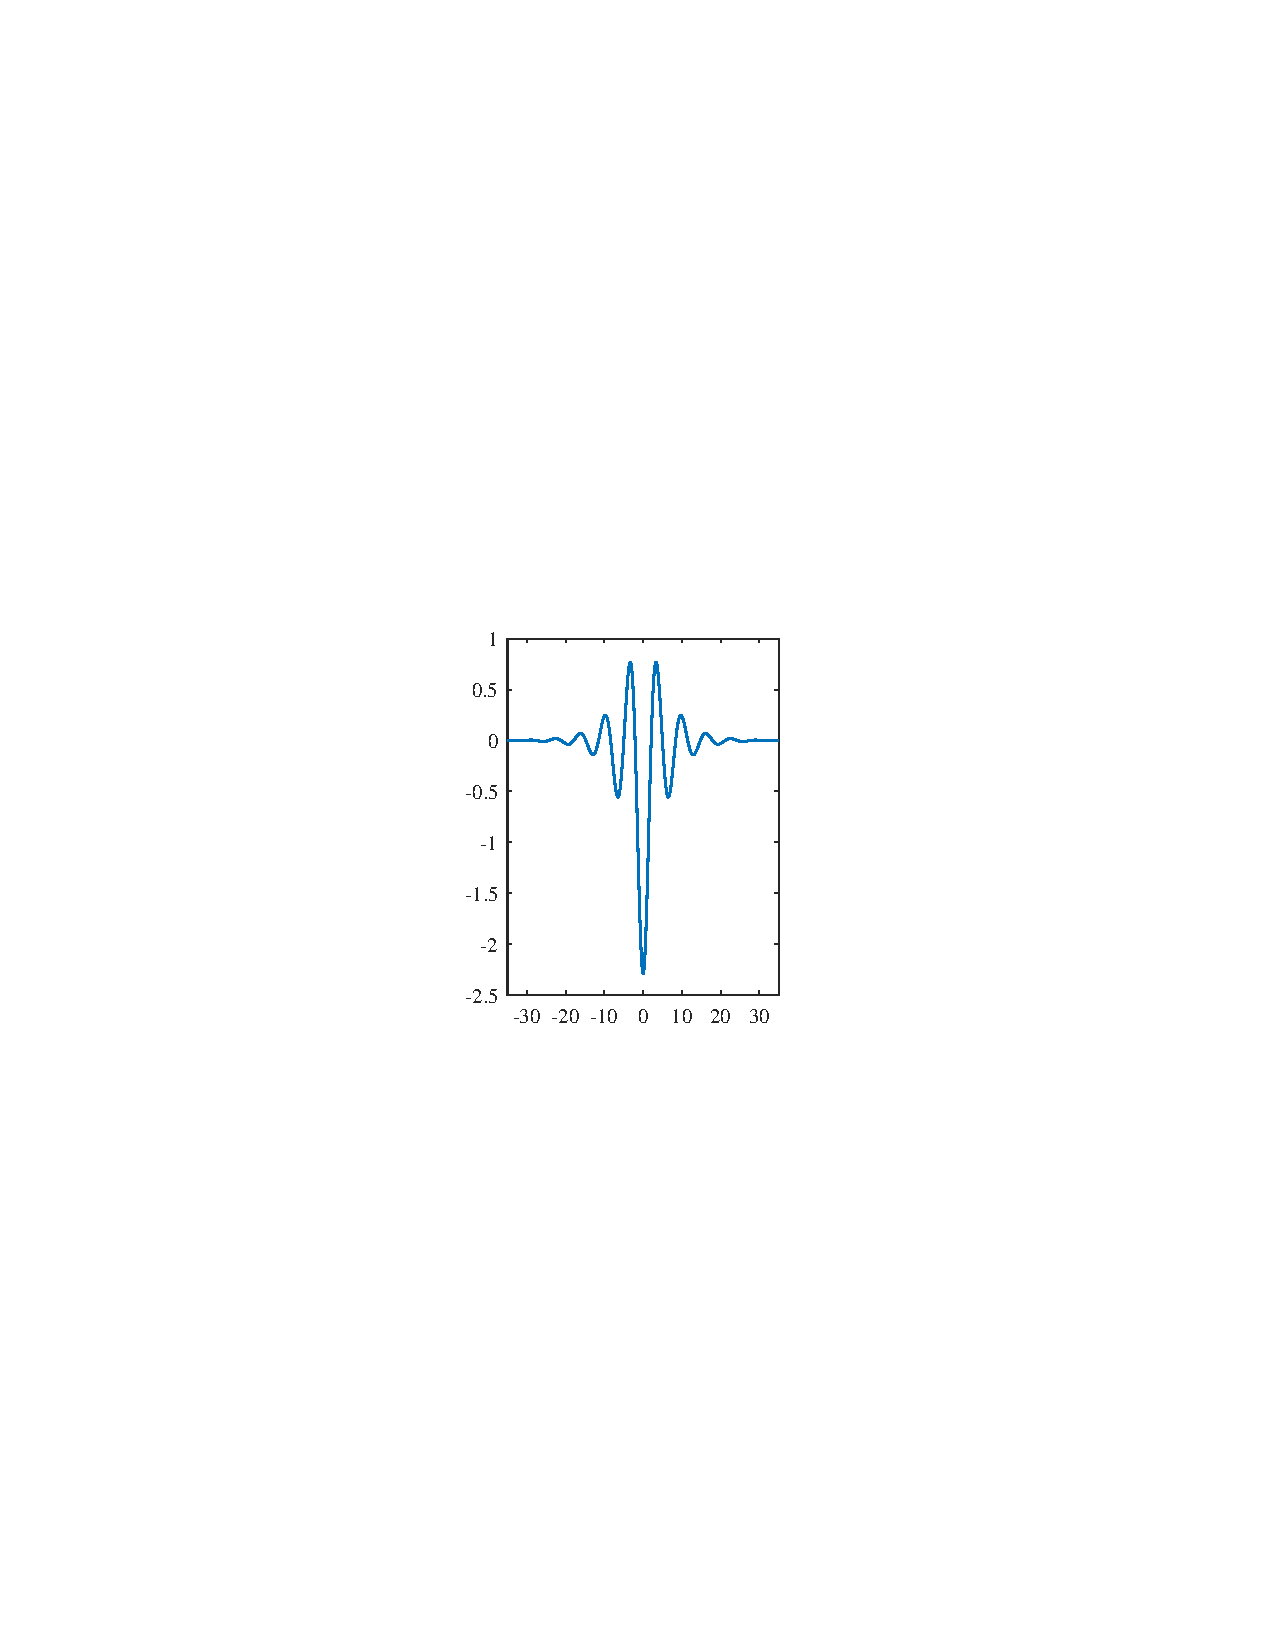
\includegraphics{images/other/single1354}&
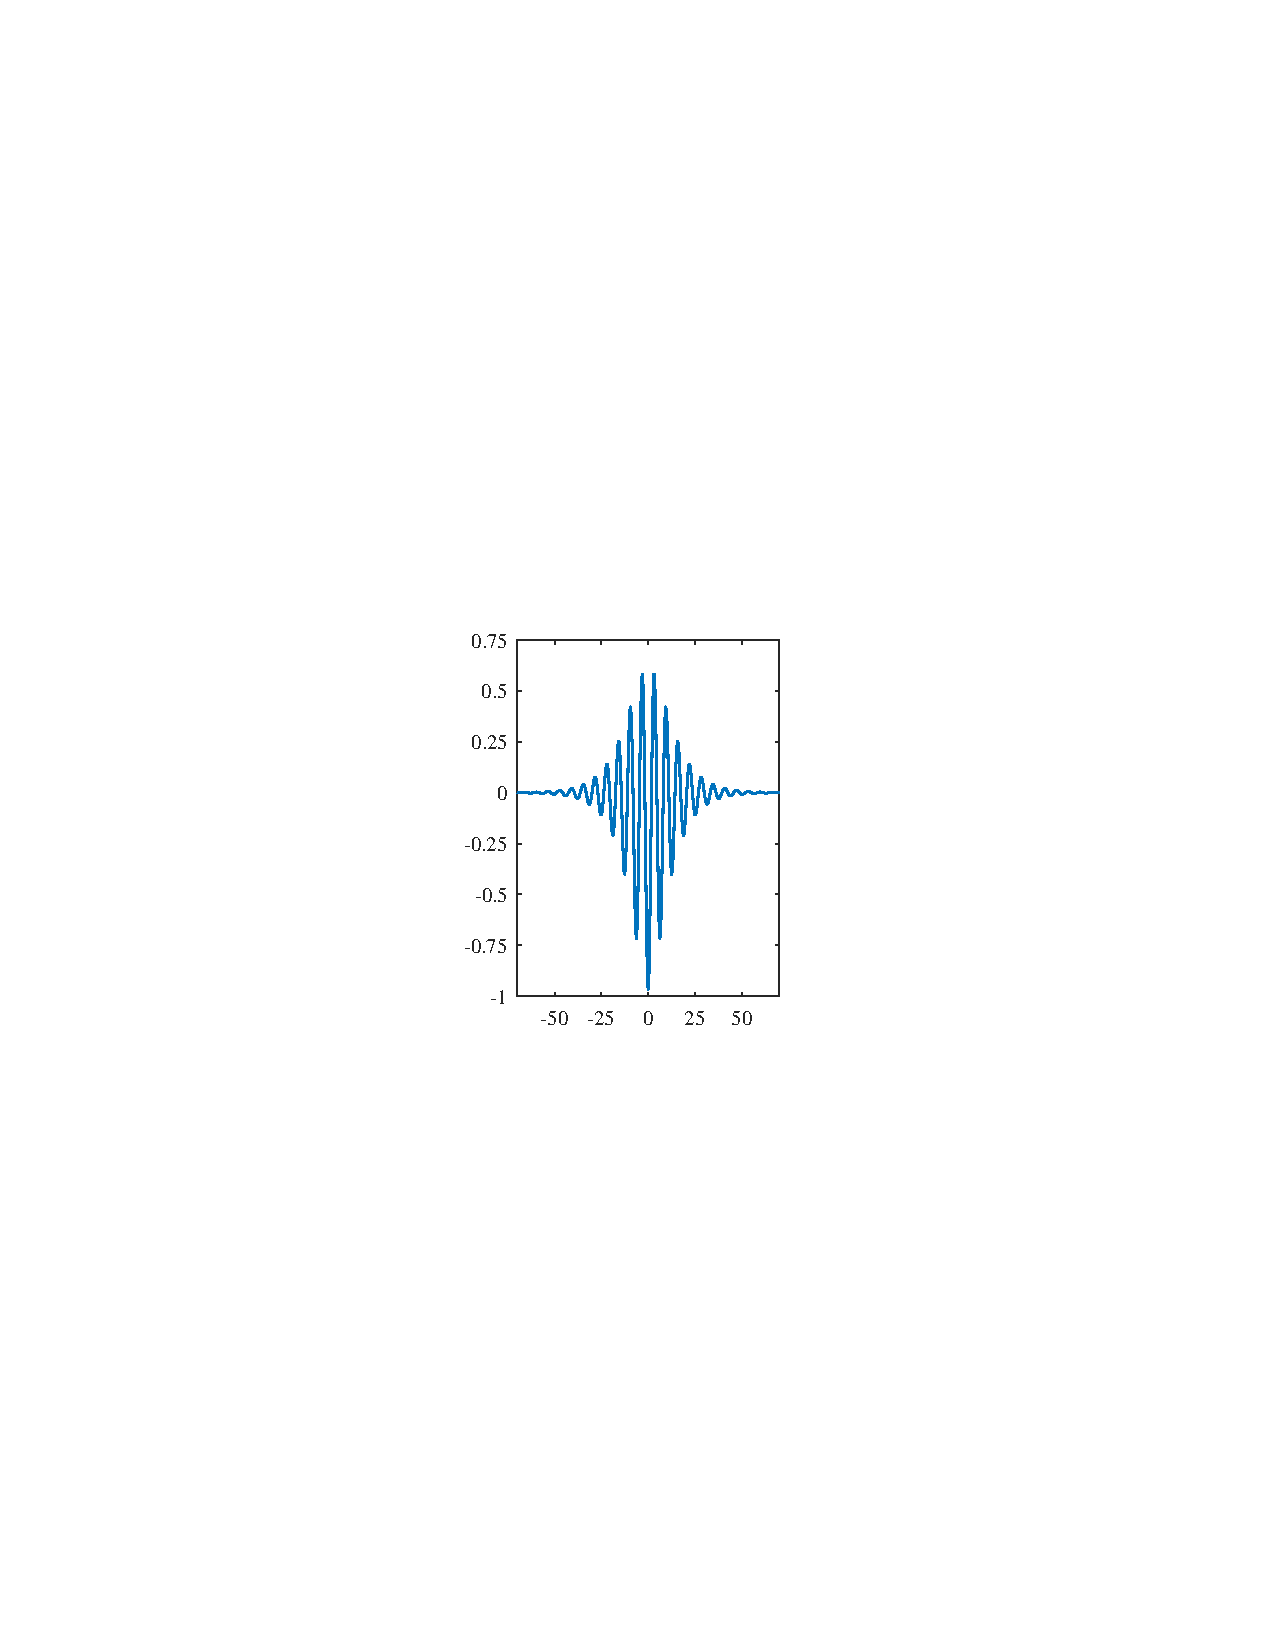
\includegraphics{images/other/single14} \\
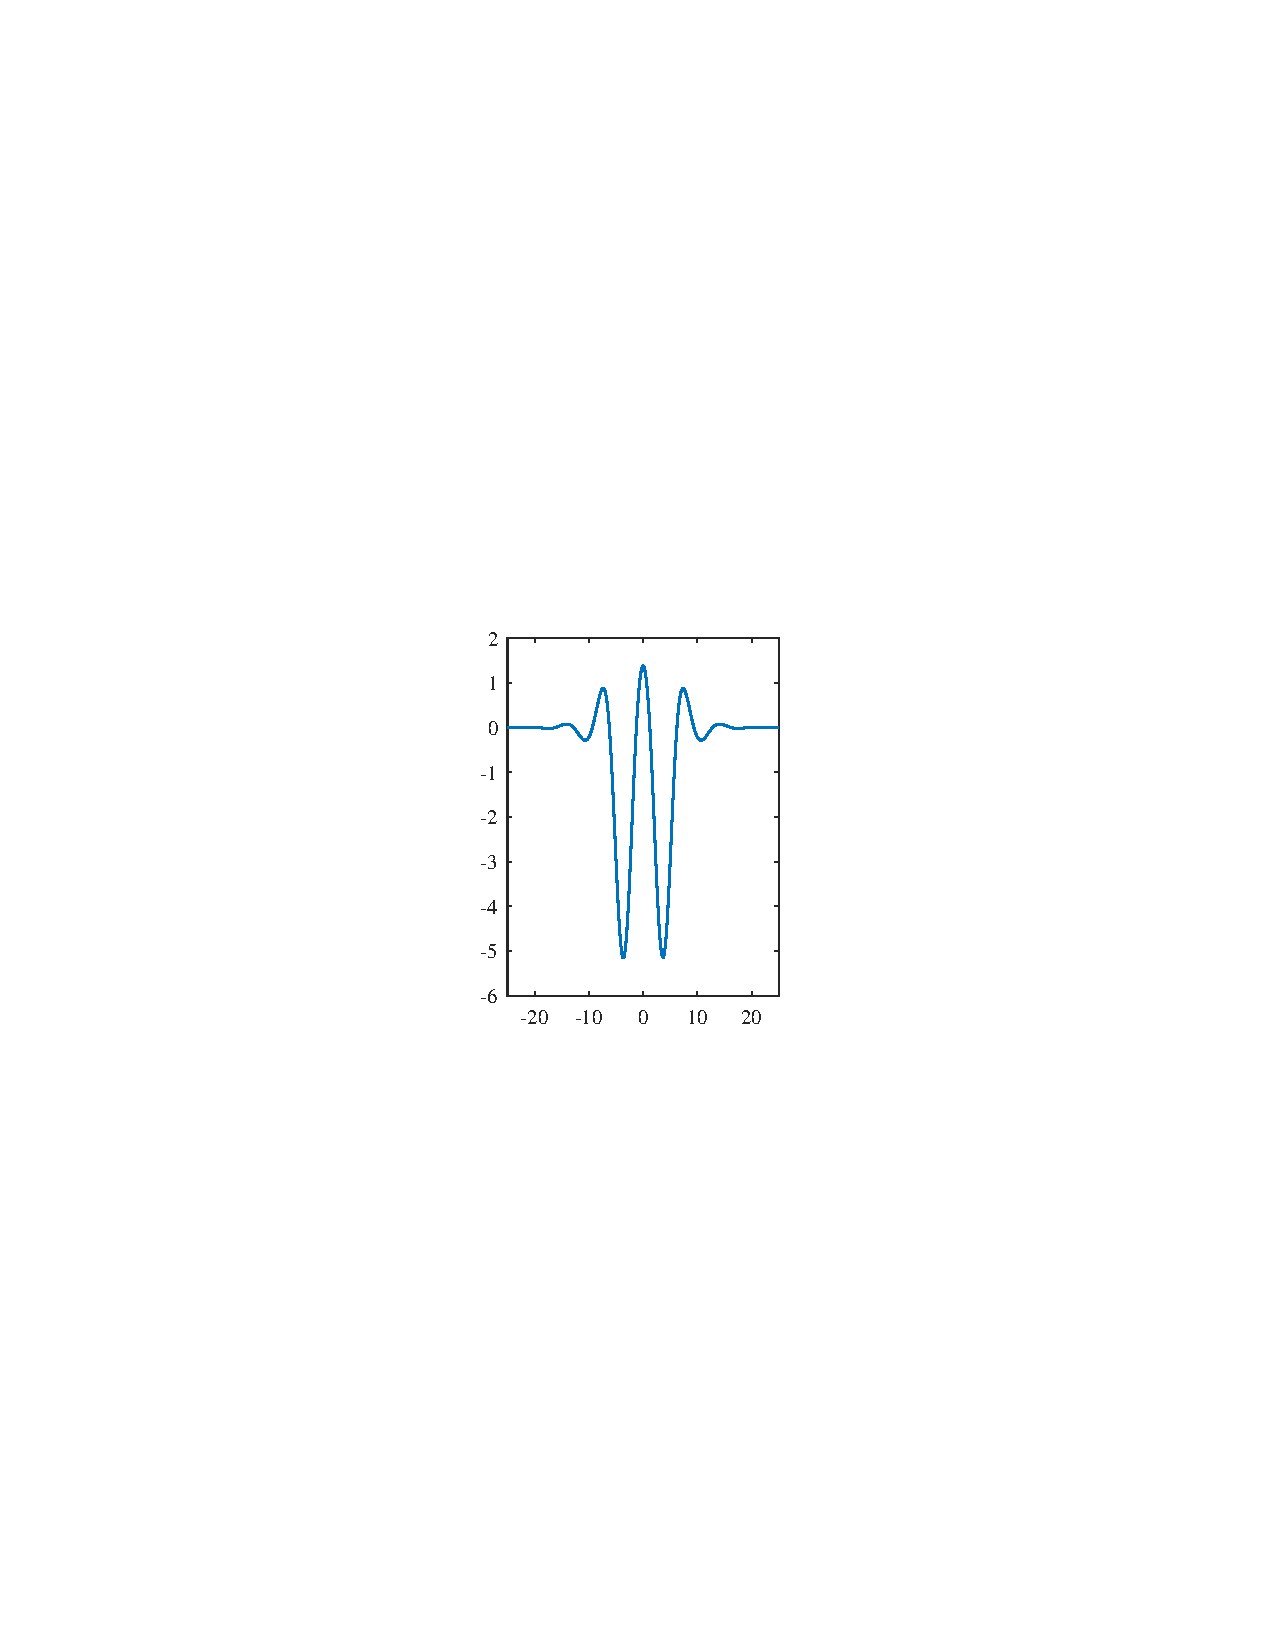
\includegraphics{images/other/double1}&
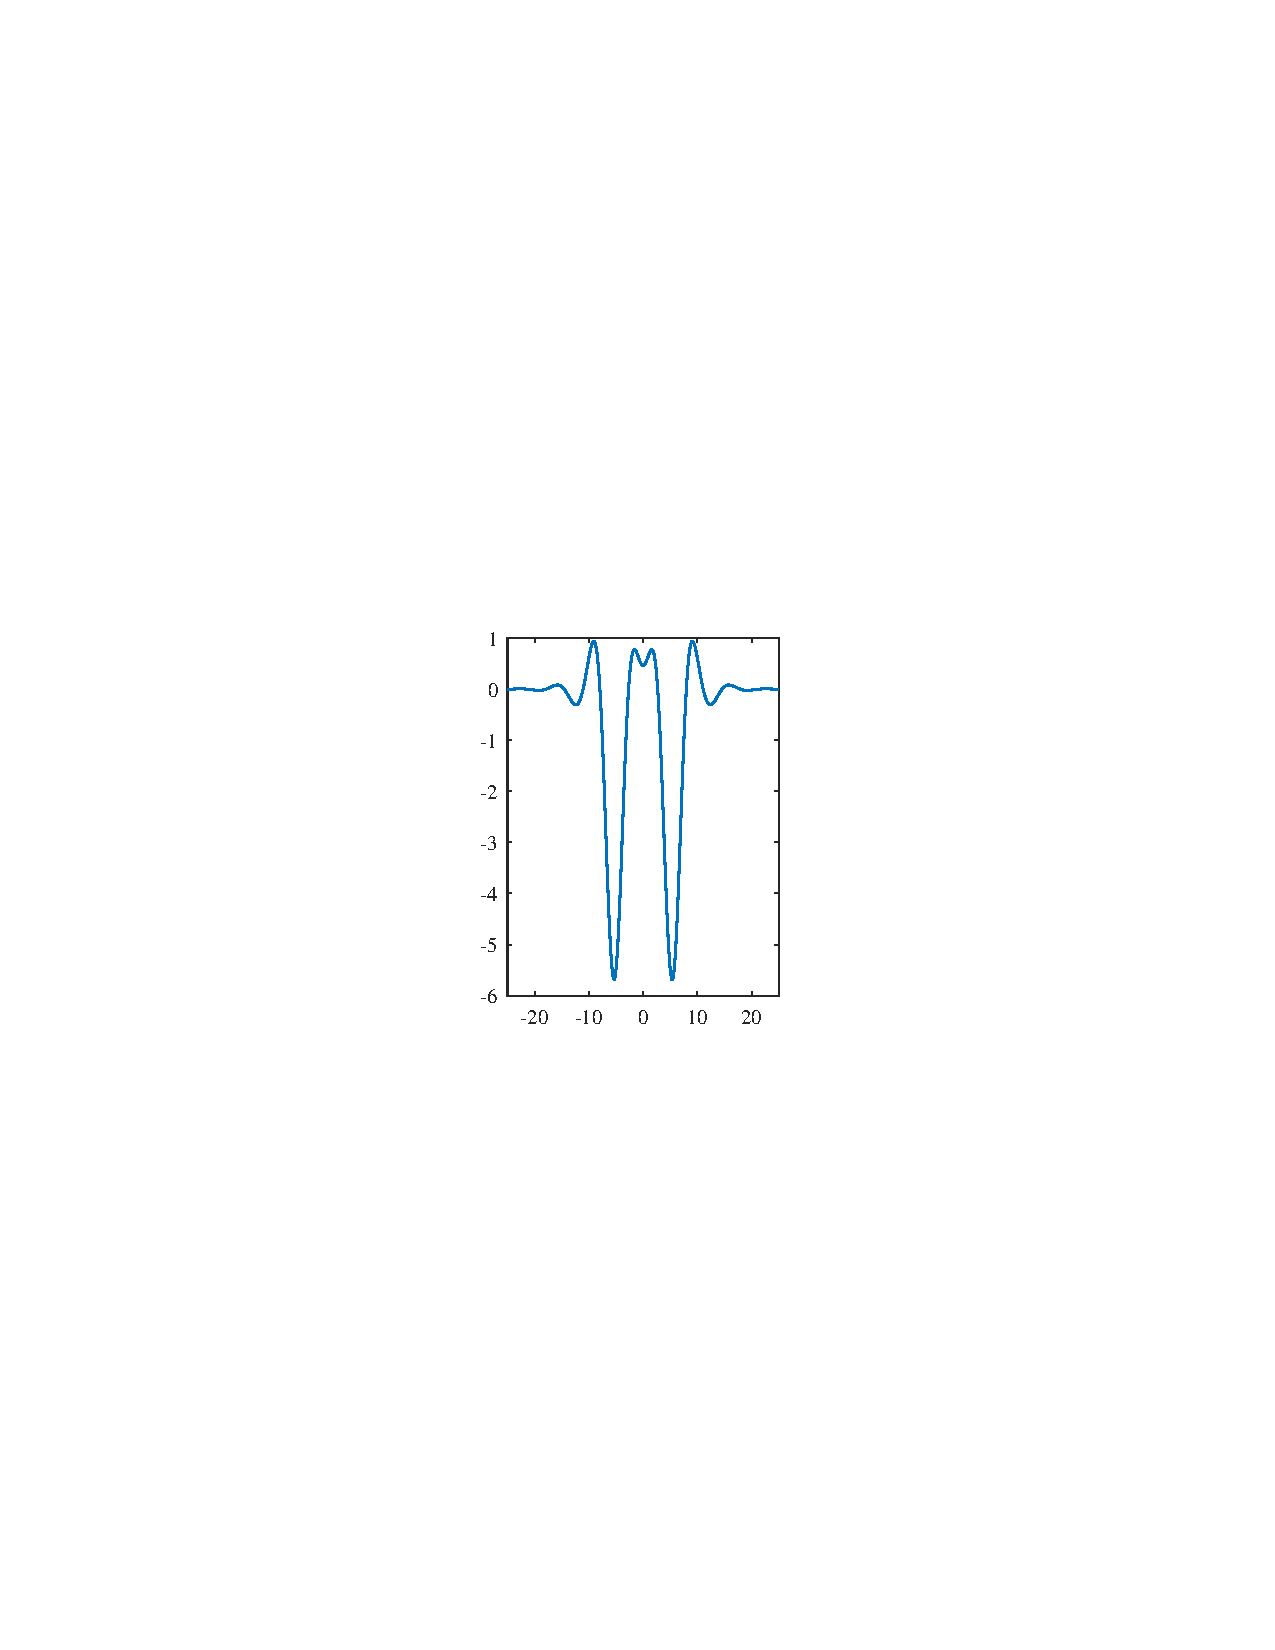
\includegraphics{images/other/double2}
\end{tabular}
\caption{Primary pulse solutions $U(x)$ to \cref{suspeq} for $c = 1.354$ (top left) and $c = 1.40$ (top right) constructed using the string method \cite{Chamard2011}. First two double pulse solutions $U_2(x)$ for $c = 1.2$ (bottom) constructed as in \cref{sec:kdv5nummulti}.}
\label{fig:chen1}
\end{figure}

We turn now to the spectral stability of multi-pulse solutions. Linearization of the PDE \cref{suspc} about a multi-pulse solution $U_n$ is the quadratic eigenvalue problem
\begin{equation}\label{quadeig}
\calI \lambda^2 - 2 c \partial_x \lambda + \calA_0(U_n) = 0,
\end{equation}
where $\calA_0(U_n)$ is defined in \cref{suspA0}. The essential spectrum of \cref{quadeig} is purely imaginary, symmetric across the real axis, and bounded away from 0. Thus for sufficiently well-separated pulses, any imaginary interaction eigenvalues will fall within the gap in the essential spectrum. Thus we avoid the issue we have with KdV5 where interaction eigenvalues may be buried in the essential spectrum. 

To determine the point spectrum, we can adapt the method in \cite{Sandstede1998} as we did in \cref{chapter:kdv5homoclinic}. Since the rest state is hyperbolic, we do not need the exponential weight. Rather than do that, in \cite{kapitula2019} we determine the spectrum using a reformulation of the Krein matrix which can be used for quadratic eigenvalue problems such as \cref{quadeig}.  Briefly, the Krein matrix is meromorphic, matrix-valued function $\vK(\lambda)$ associated with an eigenvalue problem with the property that $\det\vK(\lambda)=0$ only if $\lambda$ is a polynomial eigenvalue \cite[Theorem 3.1]{kapitula2019}. Furthermore, the Krein matrix can be used to determine the Krein signature of a purely imaginary eigenvalue. To obtain the Krein matrix, we project \cref{quadeig} onto a finite-dimensional subspace. For this problem, we choose the space $S$, which defined above after \cref{suspA0}.

In \cite[Theorem 6.8]{kapitula2019}, we prove that for an $n$-pulse solution $U_n$, the Krein matrix associated with \cref{quadeig} is diagonally dominant, thus we can determine the interaction eigenvalues from the diagonal entries of the Krein matrix. In addition, we use the Hamiltonian-Krein index, a tool which counts the potentially unstable eigenvalues, to conclude that this method locates all of the potentially unstable eigenvalues. The main result is summarized in the following theorem, which adapts \cite[Corollary 6.9]{kapitula2019} to the notation used in previous chapters.

\begin{theorem}\label{chenstab}
Assume Hypothesis \cref{chenhyp}. For $c \in (0, \sqrt{2})$, let $U(x)$ be the primary pulse solution, and let $d''(c)$ be defined as in \cref{dcc}. Let $(m_1, \dots, m_{n-1})$ be a homoclinic parameterization, and let $r_*$ be as in Theorem \ref{multipulseexistR}. For $r \in \mathcal{R}$ with $r \leq r_*$, let $U_n(x)$ be an $n-$pulse solution to \cref{suspeq}. Let $\{\mu_1, \dots, \mu_{n-1}, 0\}$ be eigenvalues of $\calA_0(U_n)$ which are close to 0. Then there are $(n-1)$ pairs of interaction eigenvalues of \cref{quadeig} which are close to 0. These are described as follows. For each $j=1,2,\dots,n-1$,
\begin{enumerate}
  \item if $m_j$ is odd (equivalently, $\mu_j<0$), there is a corresponding pair of purely imaginary interaction eigenvalues,
  \begin{equation}\label{npulseKreineigs}
	\lambda_j^\pm = \pm \rmi \left( \|\partial_xU\| \sqrt{ \frac{|\mu_j|}{d''(c)} } + \mathcal{O}(r^{3/2}) \right),
	\end{equation}
  each of which has negative Krein signature
  \item if $m_j$ is even (equivalently, $\mu_j>0$), there is a corresponding pair of real interaction eigenvalues,
   	\[
	\lambda_j = \pm \left( \|\partial_xU\| \sqrt{ \frac{\mu_j}{d''(c)} } + \mathcal{O}(r^{3/2}) \right).
	\]
  In particular, there exists a positive, real eigenvalue.
\end{enumerate}
In addition, there is a geometrically simple eigenvalue at $\lambda=0$ with corresponding eigenfunction $\partial_x U_n$. All other point spectra is purely imaginary, and has positive Krein signature.
\end{theorem}

\begin{remark}
If all the small, nonzero eigenvalues $\{ \mu_1, \dots, \mu_{n-1} \}$ of $\calA_0(U_n)$ are negative, and if the individual pulses are sufficiently well-separated, then the $n$-pulse is spectrally stable; otherwise, it is unstable.
\end{remark}

\section{Discrete nonlinear Schr{\"o}dinger equation}\label{sec:DNLS}

The discrete nonlinear Schr{\"o}dinger equation (DNLS) is the 


\begin{equation}\label{DNLS}
i\dot{\psi}_n + d(\psi_{n+1} - 2 \psi_n + \psi_{n-1}) + |\psi_n|^2 \psi_n = 0,
\end{equation}
which is (2.12) in \cite{Kevrekidis2009}, where we have taken $\beta = -1$ and $\sigma = 1$. The parameter $d$ represents the coupling between nodes; $d > 0$ is the focusing case, and $d < 0$ the defocusing case~\cite{Kevrekidis2009}. Equation \cref{DNLS} is Hamiltonian, with energy given by (2.17) in \cite{Kevrekidis2009,pelinovsky_2011}. Of general interest in this type of lattice is the existence and stability of standing waves, which are bound state solutions of the form $\psi_n(t) = e^{i \omega t}\phi_n$~\cite{alfimov}. Making this substitution in \cref{DNLS} and simplifying, a standing wave solves the steady state equation
\begin{equation}\label{DNLSequilib}
d(\phi_{n+1} - 2 \phi_n + \phi_{n-1}) - \omega \phi_n + |\phi_n|^2 u_n = 0.
\end{equation}
From~\cite{herrmann_2011}, a symmetric, real-valued, on-site soliton solution $q_n$ exists to \cref{DNLSequilib} for all $\omega \neq 0$ and $d \geq 0$. This solution $q_n$ furthermore is differentiable in $\omega$. 

We will write DNLS as a system of two real variables $u = (v, w) \in \ell^2(\Z, \R^2)$, where $v = \text{Re }\psi$ and $w = \text{Im }\psi$. In this fashion, we can write \cref{DNLS} in Hamiltonian form as
\begin{equation}\label{DNLSrealHam}
\dot{u}_n + J [\mathcal{H}'(u)]_n = 0,
\end{equation}
where $J$ is the standard skew-symmetric symplectic matrix
\[
J = \begin{pmatrix}0 & 1 \\ -1 & 0\end{pmatrix}
\]
and the Hamiltonian $\mathcal{H}: \ell^2(\Z,\R^2) \rightarrow \R$ is
\begin{equation}\label{DNLSrealH}
\mathcal{H}(v, w) = -\sum_{n = -\infty}^\infty 
\left( \frac{d}{2}\left(v_n - v_{n-1}\right)^2 + \frac{d}{2}\left(w_n - w_{n-1}\right)^2 - \frac{1}{4}\left( v_n^2 + w_n^2 \right)^2 \right).
\end{equation}
The Hamiltonian $\mathcal{H}$ is invariant under the standard rotation group $R(\theta)$, given by
\begin{equation}\label{Rtheta}
R(\theta) = \begin{pmatrix}
\cos(\theta) & \sin(\theta) \\
-\sin(\theta)& \cos(\theta)
\end{pmatrix},
\end{equation}
which has infinitesimal generator $R'(0) = J$. In addition, there is another conserved quantity, often called the norm or the power of the solution, which is given by
\begin{equation}\label{DNLSQ}
\mathcal{Q}(v, w) = \frac{1}{2} \sum_{n = -\infty}^\infty 
\left( v_n^2 + w_n ^2\right).
\end{equation}

Standing waves are solutions of \cref{DNLSrealHam} of the form $R(\omega t) u$, where $u$ is independent of $t$. Substituting this into \cref{DNLSrealHam}, we obtain the equivalent system of equations
\begin{equation}\label{DNLSequilib1}
\mathcal{H}'(u) - \omega u = 0,
\end{equation}
which for DNLS is given by
\begin{equation}\label{DNLSequilib2}
\begin{aligned}
d (v_{n+1} - 2 v_n + v_{n-1}) + v_n w_n^2 + v_n^3 - \omega v_n &= 0 \\
d (w_{n+1} - 2 w_n + w_{n-1}) + v_n^2 w_n + w_n^3 - \omega w_n &= 0 \:.
\end{aligned} 
\end{equation}
If $u$ is a standing wave solution, then $R(\theta) u$ is also a standing wave by symmetry. We note that the steady state system has the form
\begin{equation}
\mathcal{H}'(u) - \omega \mathcal{Q}'(u) = 0,
\end{equation}
which is the stationary equation \cite[(2.15)]{Grillakis1987}. The steady state equation \cref{DNLSequilib2} also has a conserved quantity $E$ \cite{Johansson2000}, which is given by
\begin{equation}\label{DNLSE}
E = 2d(v_n w_{n-1} - v_{n-1} w_n) = 2d \langle u_n, J u_{n-1} \rangle.
\end{equation}
By a conserved quantity in this setting we mean
that this quantity is independent of the lattice
index $n$.

For stability analysis, the linearization of \cref{DNLSrealHam} about a standing wave solution $u^*$ 
yields the linear operator $L(u^*)$, given by 
\begin{equation}\label{DNLSeigproblem}
L(u^*) = J \mathcal{H}''(u^*)  - \omega J.
\end{equation}
Let $u^*_n = (q_n, 0)$, where $q_n$ is the real-valued, on-site standing wave solution to \cref{DNLS}. It is straightforward to verify that
\begin{equation}\label{DNLSkernel1}
\begin{aligned}
L(u^*) R'(0) u^* &= 0 \\
L(u^*) \partial_\omega u^* &= R'(0) u^* \:.
\end{aligned}
\end{equation}
Based on these statements, we have that $0$ is an
eigenvalue with algebraic multiplicity $2$ and
geometric multiplicity $1$ in the DNLS problem.



\iffulldocument\else
	\bibliographystyle{amsalpha}
	\bibliography{thesis.bib}
\fi

\end{document}